\section{Semaine 04 (07/10-11/10) }


\e{Notions abordées :}
\begin{itemize}
	\item Équilibre chimique (cf semaine précédente).
	\item Bases de l'optique géométrique.
\end{itemize}

\subsection{Questions de cours}
\begin{enumerate}
	\item Énoncer les lois de Snell-Descartes.
	\item Définir un rayon lumineux et un MTHI.
	\item Indice de réfraction ? Phénomène de réflexion totale ?
\end{enumerate}

\subsection{Exercice 1 : Réfractomètre de Pulrich}

\begin{minipage}[c]{\linewidth/2}
	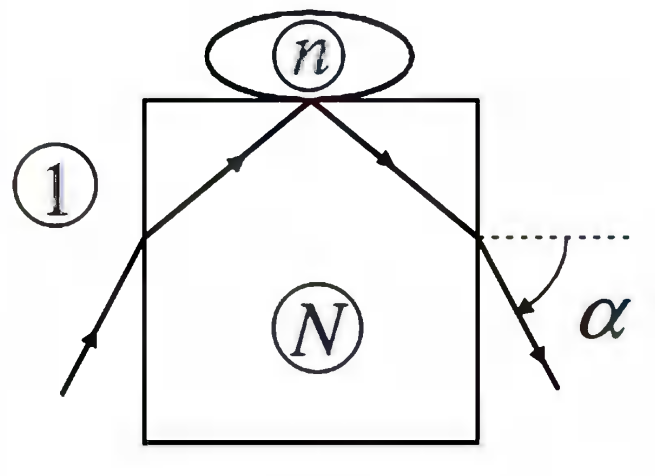
\includegraphics[width=\linewidth]{Images/mpsi_s04_ex01.png}
\end{minipage}%
\begin{minipage}[c]{\linewidth/2}
	Un réfractomètre de Pulrich est constitué d'un cube de verre d'indice $N$ connu sur lequel on a déposé une goutte d'un liquide d'indice $n$ inconnu. On observe un faisceau de rayons parallèles à la limite réfraction - réflexion totale et on mesure l'angle $\alpha$ correspondant. On donne $N=1.626$ et $\alpha=60$°.
\end{minipage} 

\begin{enumerate}
	\item Que vaut $n$ ?
	\item Quelles sont les valeurs mesurables de $n$ avec ce dispositif ?
\end{enumerate}

\e{Réponse} : $n = 1.376$

\subsection{Exercice 2}

\begin{minipage}[c]{\linewidth/2}
	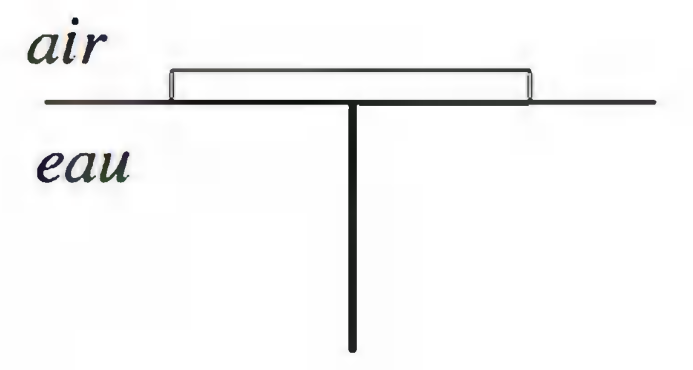
\includegraphics[width=\linewidth]{Images/mpsi_s04_ex02.png}
\end{minipage}%
\begin{minipage}[c]{\linewidth/2}
	Un disque en liège de diamètre $D = \SI{5}{cm}$ flotte sur l'eau. Il soutient une tige placée perpendiculairement en son centre. 
	
	Quelle est la longueur $h$ de la partie de la tige qu'un observateur dans l'air ne peut pas voir ?
\end{minipage}

\e{Réponse :} $h = \SI{2.1}{cm}$.

\subsection{Exercice 3 : Détection de pluie sur un pare-brise}

\begin{minipage}[c]{\linewidth/2}
	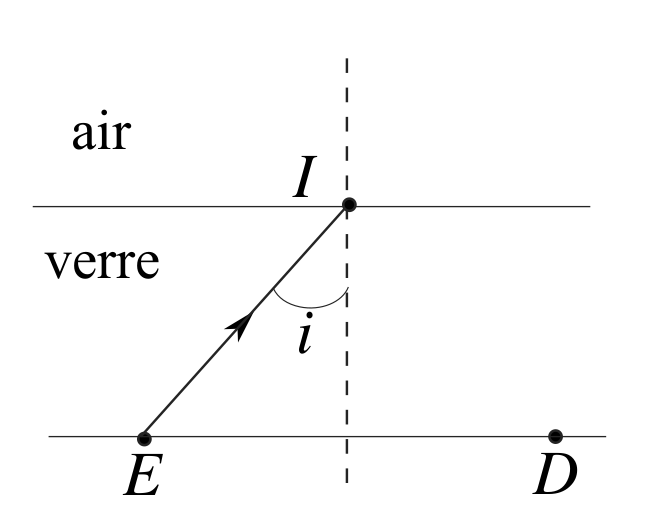
\includegraphics[width=\linewidth]{Images/mpsi_s04_ex03.png}
\end{minipage}%
\begin{minipage}[c]{\linewidth/2}
	On modélise un pare-brise par une lame de verre à faces parallèles, d'épaisseur $e = \SI{5}{mm}$, d'indice $n_v = 1.5$. Un fin pinceau lumineux issu d'un émetteur situé en $E$ arrive de l'intérieur du verre sur le dioptre verre/air en $I$ avec un angle d'incidence $i=60$°.
\end{minipage}

\begin{enumerate}
	\item Montrer que le flux lumineux revient intégralement sur le détecteur situé en $D$ et déterminer la distance $ED$.
	\item Comment ce dispositif permet-il de détecter un dépôt de pluie sur le pare-brise ? On supposera une épaisseur d'eau de $\SI{1}{mm}$.
\end{enumerate}

\e{Réponses :}
\begin{enumerate}
	\item $i_{lim} = 41.8$°.
	\item Distance au détecteur de $\SI{0.9}{cm}$.
\end{enumerate}

